\section{View to Group Classification}
\label{sec:results-grouping}
Because the grouping mechanism supplies the core functionality of the network architecture it is evaluated first.
Even if the overall performance would yield satisfiable results, but the grouping mechanism would fail the original intention, it would need to be revised.
In contrast, if the results of the network are not satisfiable, the grouping algorithm could be the cause.

The easiest case for evaluation is a single object category with three material features.
Here the network only needs to find views with a material for assigning them a high discrimination score.
It is supposed, that those views have the highest scores of all views and, hence, are members of a group with a high weight.
Views where no material is seen, should have a score close to zero, because the final prediction cannot rely on them at all.
Thus, this configuration is the most interpretable one.
The group dividing for the 0-3 network is shown in \figref{fig:grouping-0-3}.
Each number below a view refers to its score.
The text above views shows the group index with its corresponding weight.
All views appear in a ascending order by their score.
Hence, all subsequent views are part of a group until another group is mentioned.
\begin{figure}
	\centering
	\begin{subfigure}{\textwidth}
		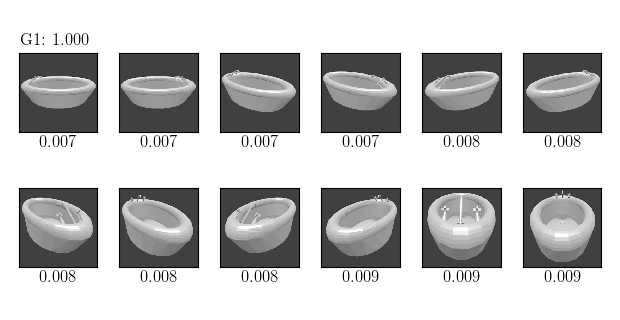
\includegraphics[trim=10 20 10 20, clip]{images/mn-sl-0-3-20/bathtub_0107_0_grouping.png}
		\caption{Blank}
		\label{fig:grouping-0-3-blank}
	\end{subfigure}
	\begin{subfigure}{\textwidth}
		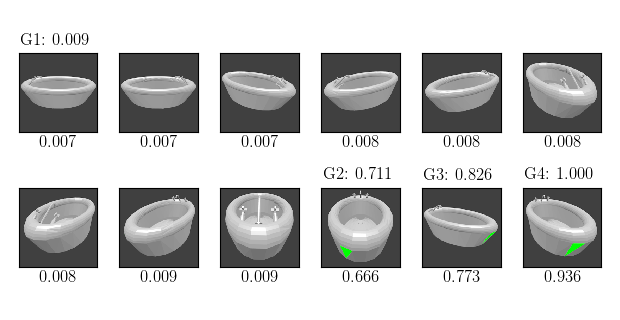
\includegraphics[trim=10 20 10 20, clip]{images/mn-sl-0-3-20/bathtub_0107_1_grouping.png}
		\caption{Green Material}
		\label{fig:grouping-0-3-green}
	\end{subfigure}
	\begin{subfigure}{\textwidth}
		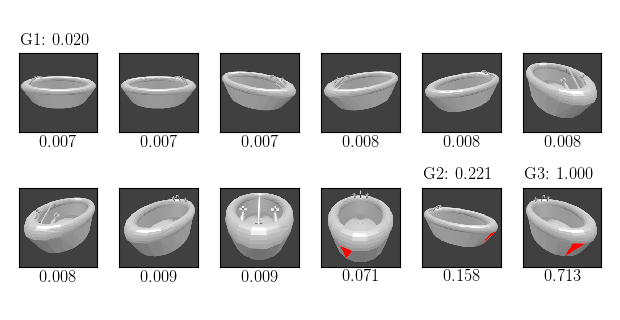
\includegraphics[trim=10 20 10 20, clip]{images/mn-sl-0-3-20/bathtub_0107_2_grouping.png}
		\caption{Red Material}
		\label{fig:grouping-0-3-red}
	\end{subfigure}
	\caption[Grouping in 0-3 Network]{Grouping in 0-3 Network}
	\label{fig:grouping-0-3}
\end{figure}
In \figref{fig:grouping-0-3-blank} a blank object is classified.
Hence, every views is similar discriminative, due to no available colored material.
Thus, the view scores are almost identical.
Those little changes presumable depend on a different weight initialization and would even out after more training epochs.
Although the scores are very low, the views are fully taken into account because they all belong to the same group with a weight of 1.
However, in this particular case a normalization of the group weight is not necessary.
Without one the group weight would be $w = 0.0079$, thus, decreasing the shape descriptor enormously, but the network would learn that a descriptor close to 0 represents a blank object.
The decision rule would be, if the descriptor represents no feature, the objects shows no feature.
With the classification of more categories, tough, this is not possible anymore, because a very small descriptor cannot just represent any blank object, but the object category class.
If there are two objects, for example, and only one view each shows a different feature with a small discrimination score, they would be divided into two categories.
Without a normalization all views would pretty much account to the same amount to the shape descriptor.
With normalization, however, the group with one view is much higher weighted than the not discriminative views.
Hence, normalization kind of removes noise, i.e. not discriminative views, that could influence the prediction unfavorably.
\figref{fig:grouping-0-3-green} and \figref{fig:grouping-0-3-red} show the expected result.
The views showing the material feature are by far the top rated views referring to their score.
It looks like, that the network prefers the slightly tilted vertical edge with a feature to its right for recognizing material features.
This exact edge is not visible in the first view showing a feature, due to the change in perspective.
Due to the mesh representation of objects, all material features are triangles.
Perhaps the dataset contains more features following this shape than in rotated ones, hence, the network focuses on that correlation.
Moreover, both figures show exactly the same order.
This shows, that the weights for each color channel are optimized in the same direction.
However, the views with the green material are in a closer range compared to the ones with the red material.
The latter differ extremely.
The least discriminative view with a material is closer to the not discriminative views than the discriminative ones.

%It is supposed, that similar views like opposite perspectives of a symmetrical object are divided into the same group, because they contain similar features.
%For example, the views of the left and right side of a car look almost identical.
%Both have the same contours but in a mirrored direction.